\section{Avvio}
\textit{Dal 2020-11-12 al 2020-12-13}

\begin{figure}[H]
	\centering
	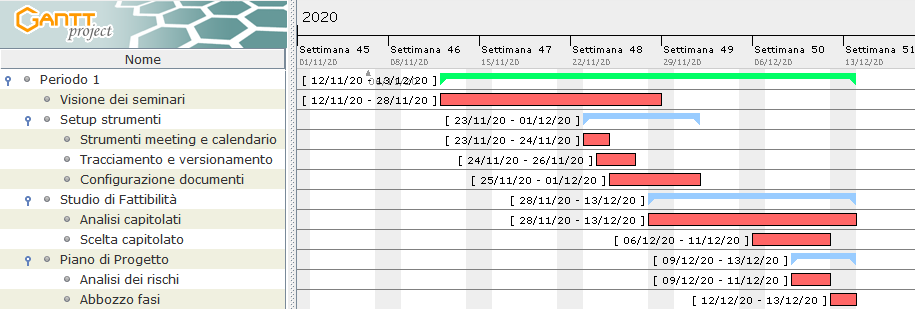
\includegraphics[scale=0.62]{res/images/gantt_fase/01_gantt_avvio.png}
	\caption{Diagramma di Gantt\textsubscript{G} relativo alla fase\textsubscript{G} di Avvio}
\end{figure}


\subsection{Periodo 1}

\subsubsection{Pianificazione preventiva}



\paragraph{Attività}
\subparagraph*{}

\planningTable{
	Visione dei seminari & I seminari tecnologici costituiscono un fattore importante nel contesto della scelta del capitolato, fanno luce sui requisiti e sulla fattibilità dei progetto & 10 & Analista
\tabularnewline 
Setup strumenti & Si studiano e testano gli strumenti che permetteranno l'organizzazione interna, il tracciamento, la stesura dei documenti e il loro versionamento, la gestione dei meeting e la loro calendarizzazione & 8 & Amministratore
\tabularnewline 
Studio di Fattibilità & L'analisi del materiale di ogni capitolato\textsubscript{G} permette al gruppo di farsi una prima idea sui punti di forza e sulle criticità di ognuno & 14 & Analista
\tabularnewline 
Piano di Progetto & Inizia la redazione del \textsc{Piano di Progetto} nelle sue parti fondamentali, a partire da una prima definizione delle fasi\textsubscript{G} e dei rischi & 14 & Responsabile
\tabularnewline 
Verifica artefatti & Vengono verificati i documenti prodotti & 10 & Verificatore
\tabularnewline 
\caption{Pianificazione preventiva - Avvio - Periodo 1}
}



\paragraph{Preventivo}
\subparagraph*{}

\hspace{-1cm}
\begin{minipage}{0.60\textwidth}
	\smallPreventivoTable{	Responsabile & 14 & 420\\ 
Verificatore & 10 & 150\\ 
Analista & 24 & 600\\ 
Amministratore & 8 & 160\\ 
Programmatore & 0 & 0\\ 
Progettista & 0 & 0\\ 
\hlinetable 
\textbf{Totale} & \textbf{56} & \textbf{1330}\\ 
\end{tabular} 
\caption{Preventivo - Avvio - Periodo 1}
}
\end{minipage}
\begin{minipage}{.40\textwidth}
\begin{figure}[H]
	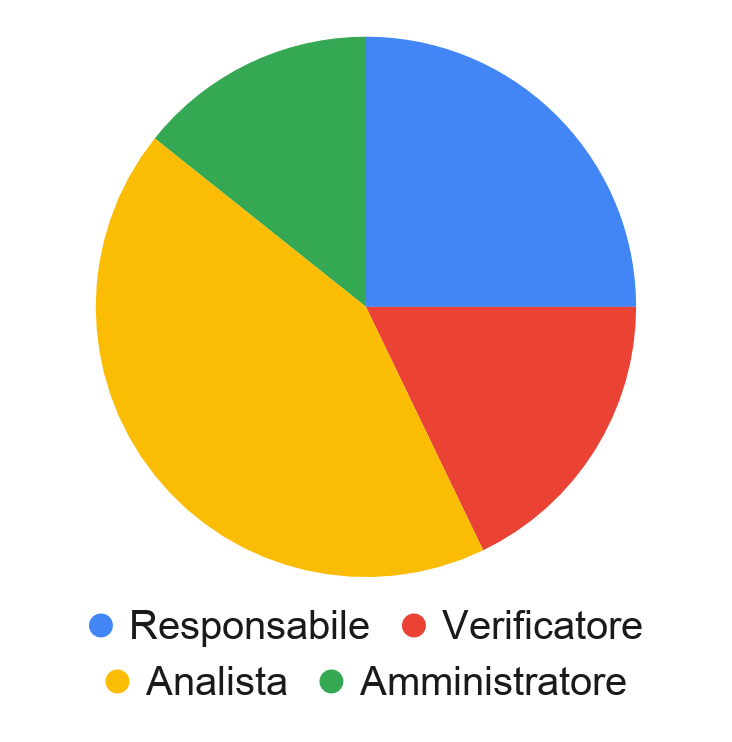
\includegraphics[scale=0.21]{res/images/charts/preventivo_priori/Grafico4-0.png}
	\caption{Distribuzione dei costi: preventivo - Avvio - Periodo 1}
\end{figure}
\end{minipage} 


\subsubsection{Pianificazione di periodo}

\paragraph{Preventivo orario ed economico}
\subparagraph*{}

\contabilitaTable{
	Chiarello Sofia & 2 & 2 & 5 & 0 & 0 & 0 & \textbf{9}\\ 
Crivellari Alberto & 2 & 2 & 5 & 0 & 0 & 0 & \textbf{9}\\ 
De Renzis Simone & 4 & 1 & 2 & 3 & 0 & 0 & \textbf{10}\\ 
Greggio Nicolò & 2 & 1 & 2 & 5 & 0 & 0 & \textbf{10}\\ 
Tessari Andrea & 2 & 2 & 5 & 0 & 0 & 0 & \textbf{9}\\ 
Zuccolo Giada & 2 & 2 & 5 & 0 & 0 & 0 & \textbf{9}\\ 
\hlinetable 
\textbf{Totale orario} & \textbf{14} & \textbf{10} & \textbf{24} & \textbf{8} & \textbf{0} & \textbf{0} & \textbf{56}\\ 
\textbf{Totale costo} & \textbf{420} & \textbf{150} & \textbf{600} & \textbf{160} & \textbf{0} & \textbf{0} & \textbf{1330}\\ 
\end{tabular} 
\caption{Preventivo di periodo - Avvio - Periodo 1}
}

\begin{figure}[H]
	\centering
	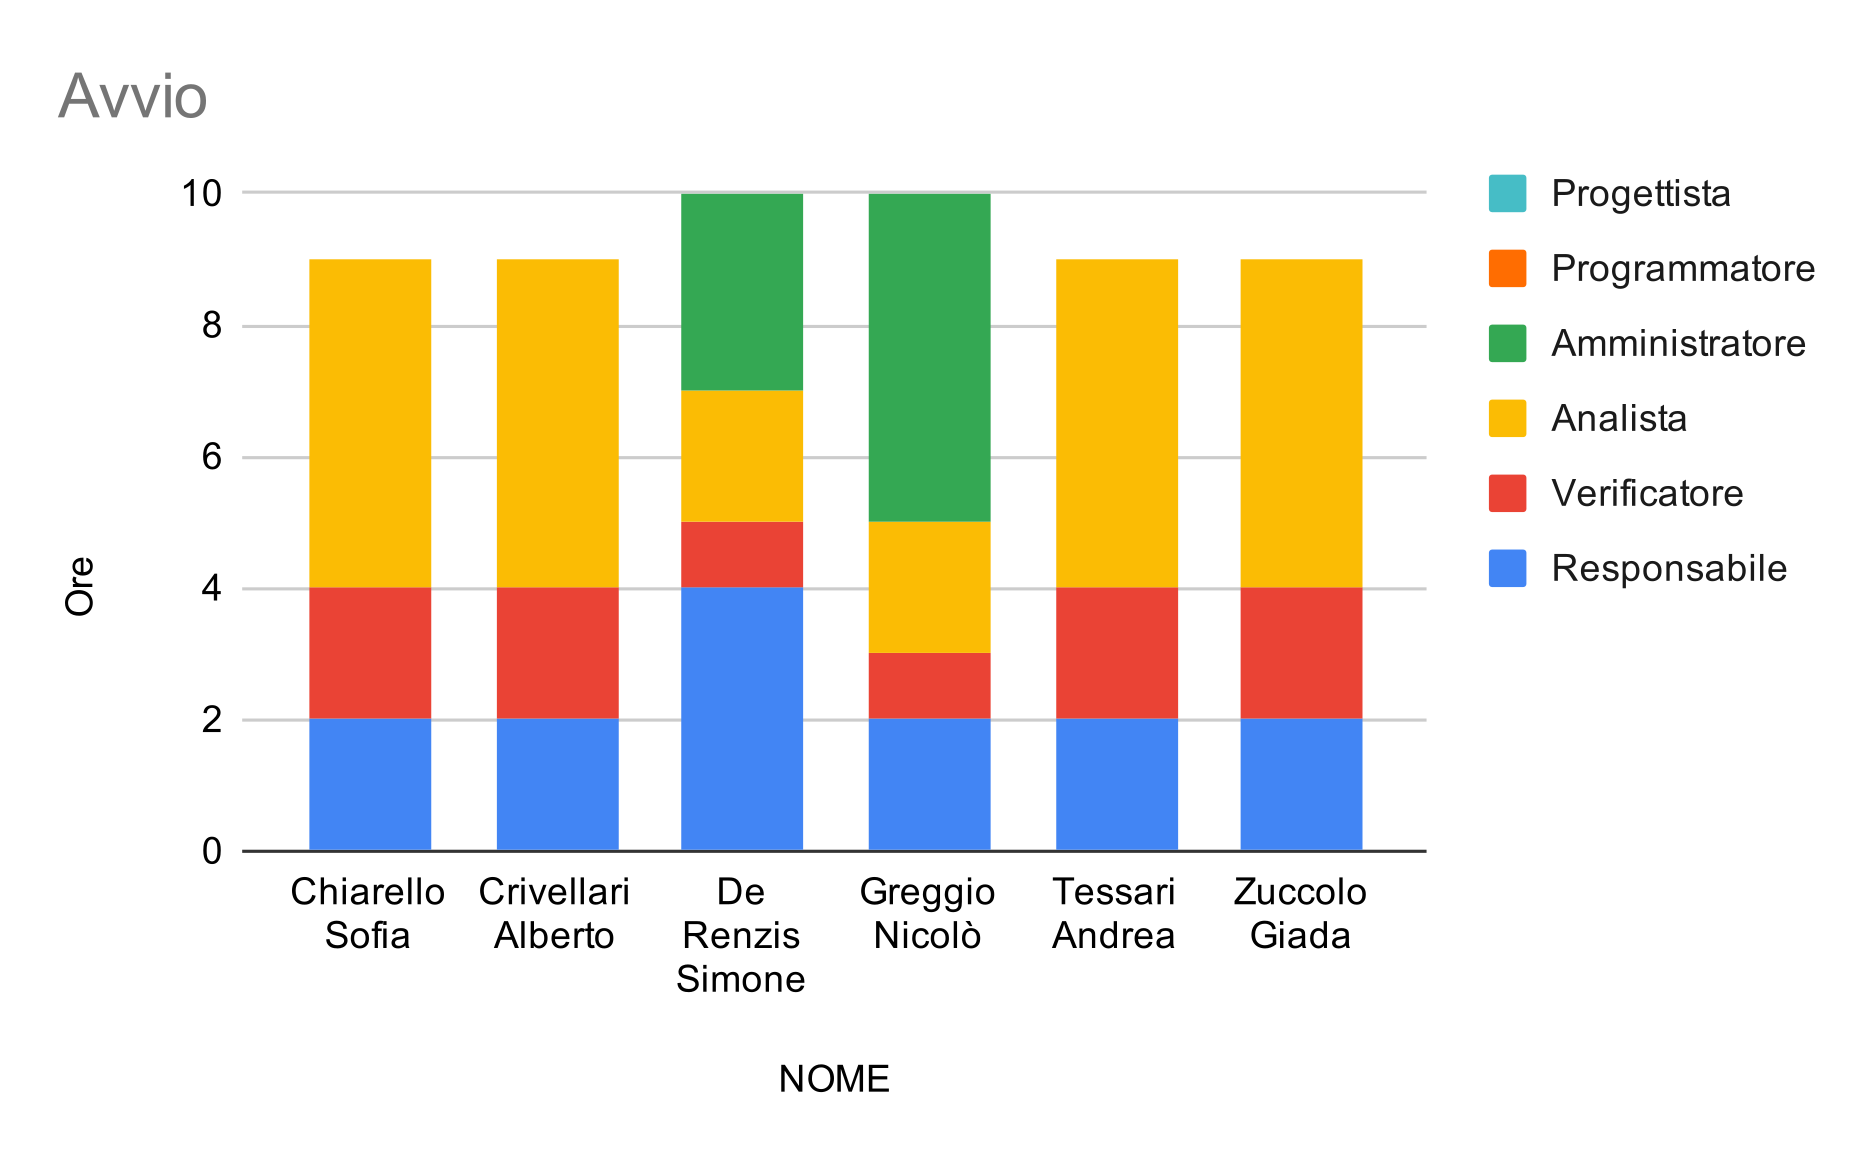
\includegraphics[scale=2]{res/images/charts/preventivo/avvio.png}
	\caption{Distribuzione oraria per componente: preventivo di periodo\textsubscript{G} - Avvio - Periodo 1}
\end{figure}

\subsubsection{Riscontro di fine periodo}

\paragraph{Consuntivo orario ed economico}
\subparagraph*{}

\contabilitaTable{
	Chiarello Sofia & 1 & 0 & 4 & 3 & 0 & 0 & \textbf{8} \\ 
Crivellari Alberto & 2 & 0 & 1 & 2 & 0 & 0 & \textbf{5} \\ 
De Renzis Simone & 3 & 0 & 2 & 4 & 0 & 0 & \textbf{9} \\ 
Greggio Nicolò & 2 & 0 & 2 & 5 & 0 & 0 & \textbf{9} \\ 
Tessari Andrea & 2 & 0 & 1 & 3 & 0 & 0 & \textbf{6} \\ 
Zuccolo Giada & 1 & 0 & 4 & 2 & 0 & 0 & \textbf{7} \\ 
\hlinetable 
\textbf{Totale orario} & \textbf{11} & \textbf{0} & \textbf{14} & \textbf{19} & \textbf{0} & \textbf{0} & \textbf{44} \\ 
\textbf{Differenza orario} & \textbf{-3} & \textbf{-10} & \textbf{-10} & \textbf{11} & \textbf{0} & \textbf{0} & \textbf{-12} \\ 
\textbf{Totale costi} & \textbf{330} & \textbf{0} & \textbf{350} & \textbf{380} & \textbf{0} & \textbf{0} & \textbf{1060} \\ 
\textbf{Differenza costi} & \textbf{-90} & \textbf{-150} & \textbf{-250} & \textbf{220} & \textbf{0} & \textbf{0} & \textbf{-270} \\ 
\end{tabular} 
\caption{Consuntivo - Avvio - Periodo 1}
}

\begin{figure}[H]
	\centering
	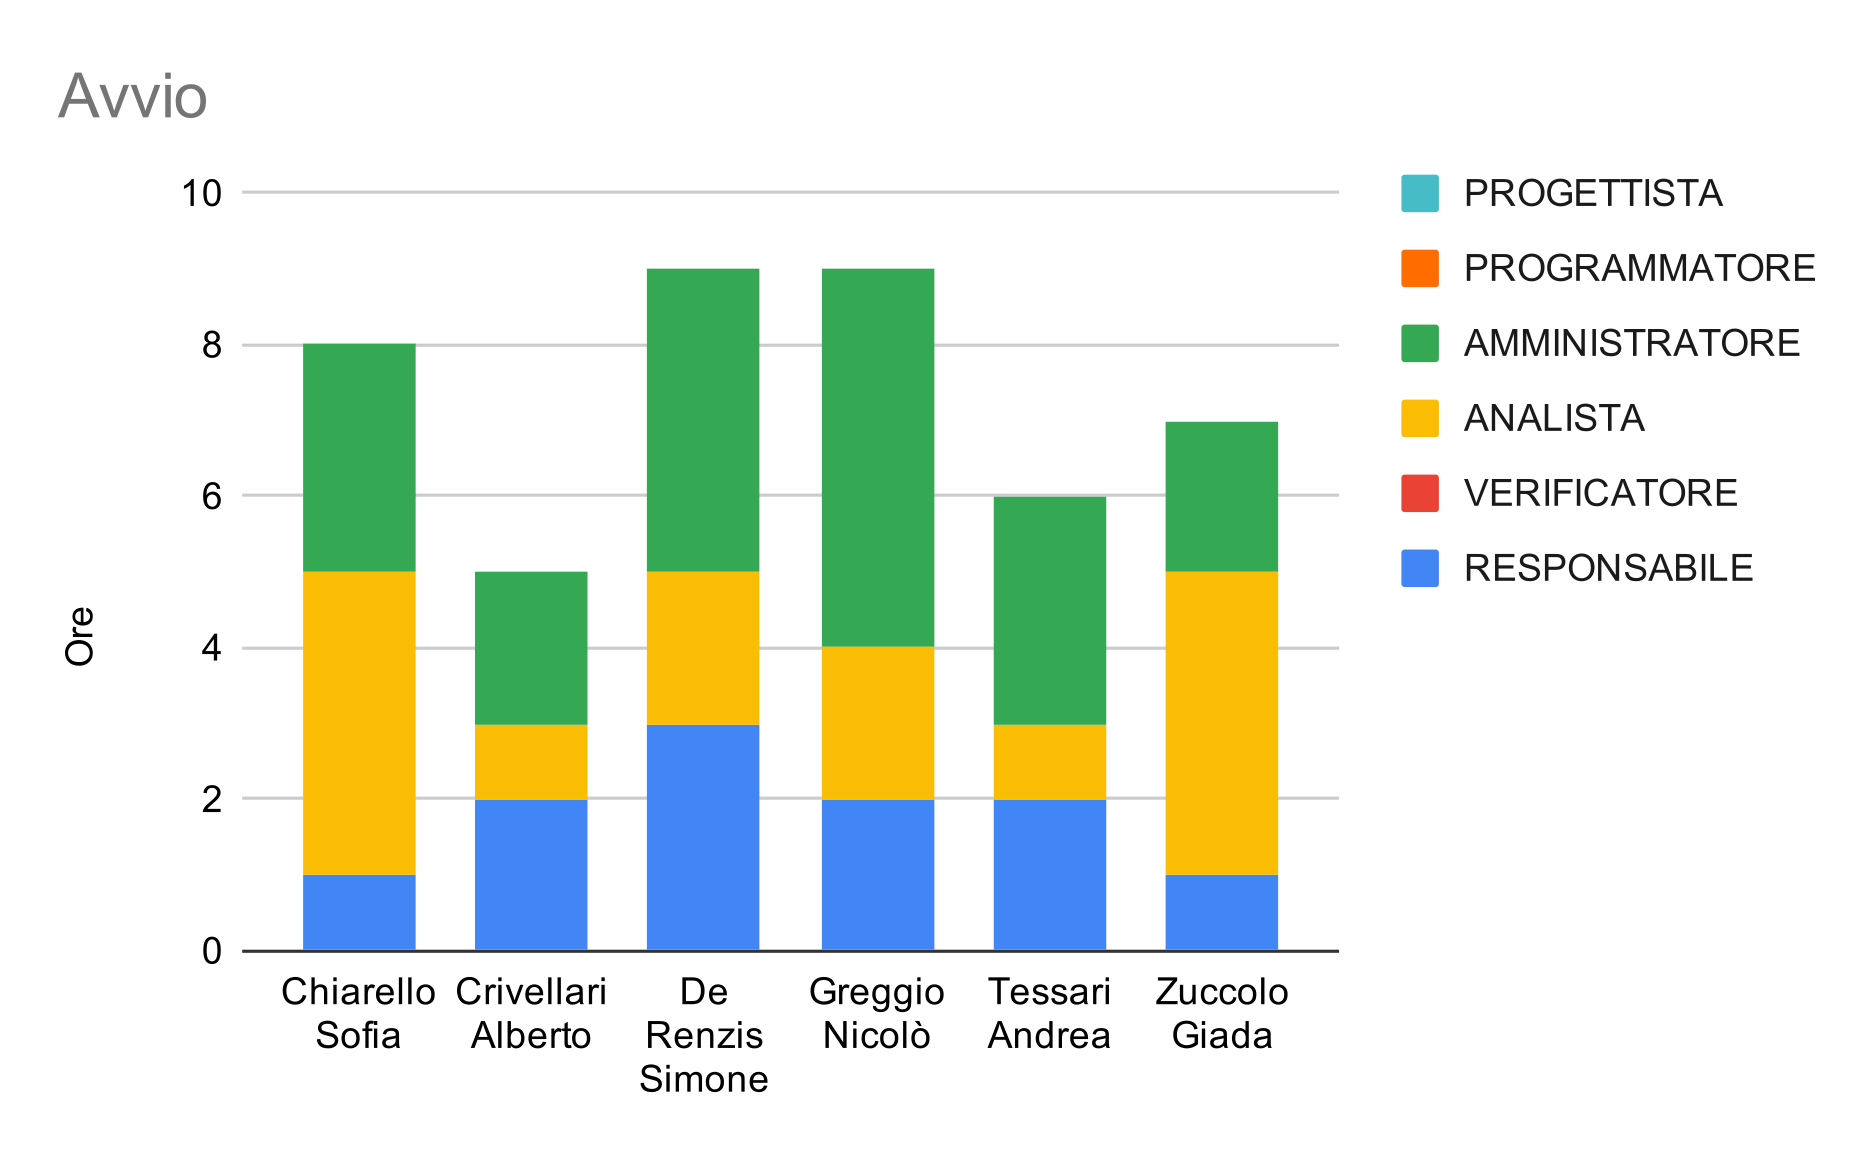
\includegraphics[scale=2]{res/images/charts/consuntivo/avvio.png}
	\caption{Distribuzione oraria per componente: consuntivo - Avvio - Periodo 1}
\end{figure}

Il periodo\textsubscript{G} chiude in \textbf{positivo}, con un risparmio di \textbf{270 \euro}. L'organizzazione del Way of Working e la messa a punto degli strumenti è proceduta in maniera più veloce del previsto.


\paragraph{Preventivo a finire}
\subparagraph*{}

\pafTable{
	Avvio & 1 & Consuntivo & 
\tabularnewline
Analisi dei Requisiti & 1 & Preventivo & 3085
\tabularnewline
Analisi dei Requisiti & 2 & Preventivo & 230
\tabularnewline
Progettazione Architetturale & 1 & Preventivo & 680
\tabularnewline
Progettazione Architetturale & 2 & Preventivo & 2414
\tabularnewline
Progettazione Architetturale & 3 & Preventivo & 280
\tabularnewline
Progettazione di Dettaglio e Codifica & 1 & Preventivo & 1270
\tabularnewline
Progettazione di Dettaglio e Codifica & 2 & Preventivo & 4097
\tabularnewline
Progettazione di Dettaglio e Codifica & 3 & Preventivo & 258
\tabularnewline
Validazione e Collaudo & 1 & Preventivo & 220
\tabularnewline
Validazione e Collaudo & 2 & Preventivo & 2145
\tabularnewline
Validazione e Collaudo & 3 & Preventivo & 60
\tabularnewline
\textbf{Totale} & \textbf{} & \textbf{} & \textbf{14739}
\tabularnewline
\textbf{Totale rendicontato} & \textbf{} & \textbf{} & \textbf{10744}
\tabularnewline
\caption{Preventivo a finire - Avvio - Periodo 1}
}

